%        File: covo.tex
%     Created: Di Okt 16 10:00  2018 C
% Last Change: Di Okt 16 10:00  2018 C
%

\documentclass[a4paper]{report}
% ***************************PACKAGES***************************
\usepackage{graphicx}
\usepackage{caption,setspace}
\usepackage{subcaption}
\captionsetup[figure]{width=0.7\textwidth,font={small}}
\usepackage{float}
\usepackage{amsmath}
\usepackage{amssymb}
\usepackage{hyperref}
\usepackage{siunitx}
\usepackage{graphicx}
\usepackage{subcaption}
\usepackage{mwe}
\usepackage{tabularx}
\usepackage{cite}
\usepackage{hyperref}
\usepackage{bookmark}


% ***************************CONFIGS***************************
% for numbering per section
\numberwithin{figure}{section}
% removing ugly colored rectangles from references
\usepackage{xcolor}
\hypersetup{
    hidelinks,
    colorlinks = false,
    %linkcolor={black},
    %citecolor={black},
    %urlcolor={black}
  }
% command for table tabular alignment
\newcolumntype{L}{>{\raggedright\arraybackslash}X}
% command for argmin and argmax
\DeclareMathOperator*{\argmax}{arg\,max}
\DeclareMathOperator*{\argmin}{arg\,min}
\newcommand{\R}{\mathbb{R}}
% commands for cascading subfigures
\newsavebox{\subfloatbox}
\newcommand{\topfloat}[2][\empty]% #1 = caption, #2=image
 {\savebox\subfloatbox{#2}%
  \begin{minipage}[t]{\wd\subfloatbox}
    \usebox\subfloatbox
    \subcaption{#1}
  \end{minipage}}
\newcommand{\bottomfloat}[2][\empty]% #1 = caption, #2=image
 {\savebox\subfloatbox{#2}%
  \begin{minipage}[b]{\wd\subfloatbox}
    \captionsetup{position=top}%
    \subcaption{#1}
    \usebox\subfloatbox
  \end{minipage}}



% ***************************ACRONYMS***************************
\usepackage[toc, shortcuts]{glossaries}
\makeglossaries
\newacronym{vo}{VO}{Visual Odometry}



\begin{document}

% ***************************TITLE***************************
\begin{titlepage}
\begin{center}

%  
\includegraphics[width=\textwidth]{../fig/tuc_logo.jpg}

\vspace{1.5cm}


{\Huge \textbf{Master Thesis}}\\
\vspace{0.5cm}
{\huge \textbf{An Error Aware RGB-D \\Visual Odometry}}


\vspace{2.5cm}

{\huge \textbf{U\u{g}ur Bolat}}

\vfill

Date:

\vspace{1.2cm}

Supervisors: \\
Dr.-Ing. Sven Lange \\
M.Sc. Tim Pfeifer

\vspace{0.8cm}

Faculty of Electrical Engineering and Information Technology\\
Professorship of Process Automation

\end{center}
\end{titlepage}

% ***************************TABLE OF CONTENT ETC.***************************
\tableofcontents
\newpage
\listoffigures
\listoftables
\newpage
\printglossary[type=\acronymtype,title={Abbreviations}]
\newpage

% ***************************DOCUMENT***************************

\begin{abstract}


\end{abstract}

\newpage

% ***************************CP1-INTRO***************************
\chapter{Introduction} \label{cp_intro}


\newpage

% ***************************CP2-VO***************************
\chapter{Visual Odometry} \label{cp_vo}

\section{Related Works} \label{sc_related_works}

\section{Camera Models} \label{sc_cam_models}

A camera maps from a 3D world scene to a 2D image plane. We call this process 
projection operation. Since the \acrshort{vo} systems process camera image 
sequences, one has to model this projection operation accurately. One of the 
basic camera modeling technique is the \textit{Pinhole Model} where the projection of 
the 3D points are mapped on a 2D image plane (also called focal plane). 

\subsection{The Pinhole Model} \label{sbsc_pinhole}

In this model, the camera centre sits behind the image plane.
The Z-axis, 
also called \textit{principal axis}, of this 
coordinate system points out through the origin of the image plane and the 
point where pierce through image plane is called the \textit{pricipal point}. 
We can also see how other two axes are located in Figure-\ref{fig:pinhole} 
and this is known as the \textit{Camera Coordinate System} $(x_{cam}, y_{cam}, z_{cam})$.


\begin{figure}[H]
	\centering
	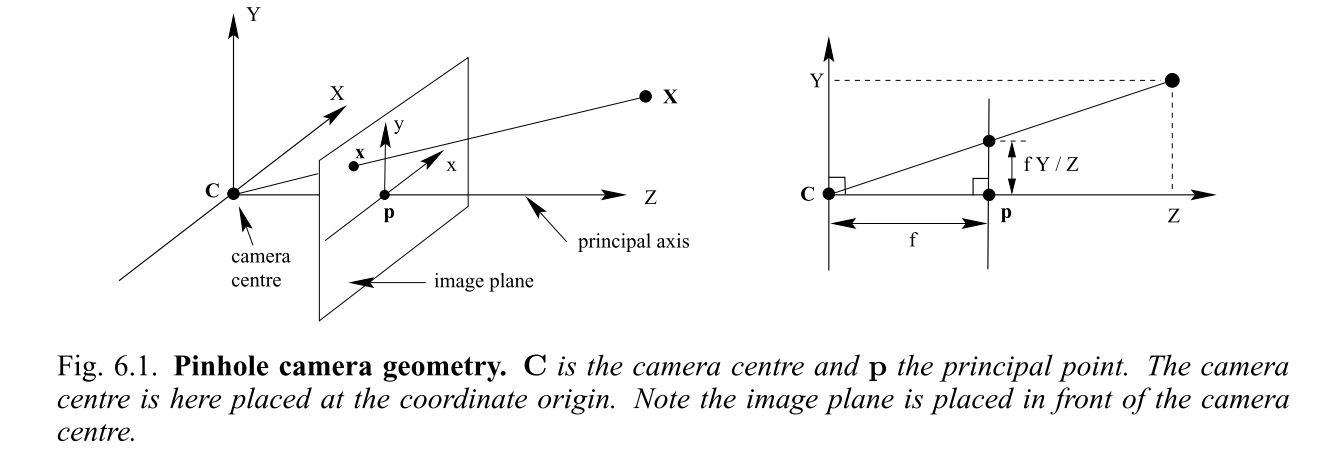
\includegraphics[width=\linewidth,natwidth=640,natheight=640]
  {fig/unofficial/pinhole_model.png}
  \caption{REMEMBER TO DRAW HORIZ/VERT Fx and Fy. The Pinhole Model}
	\label{fig:pinhole}
\end{figure}

Thanks to geometrical propotion property, we can project 
the 3D point $(X, Y, Z)^T$ in Euclidean space $\mathbb{R}^3$
to the 2D point $(U,V)^T = (f_xX/Z, f_yY/Z)^T$ in Euclidean space $\mathbb{R}^2$, 
where $f_x$ and $f_y$ are the \textit{focal lengths} 
between the camera centre and the pricipal 
point with respect to horizontal and vertical axis of the Camera Coordinate 
System respectively.
After projection, we obtain a 2D 
point that we represent on the 
\textit{Image Coordinate Frame} $(u_{img},v_{img})$.

To be more specific,
we can write the projection operation as a linear mapping function 
in the following way if we utilize the homogenous coordinates:

\begin{equation}
  \begin{pmatrix}
    U\\
    V\\
    1
  \end{pmatrix}
  =
  \begin{pmatrix}
    f_xX/Z\\
    f_yY/Z\\
    1
  \end{pmatrix}
  =
  \begin{pmatrix}
    f_xX\\
    f_yY\\
    Z
  \end{pmatrix}
  =
  \begin{bmatrix}
    f_x & 0 & 0 & 0\\
    0 & f_y & 0 & 0\\
    0 & 0 & 1 & 0\\
  \end{bmatrix}
  \begin{pmatrix}
    X\\
    Y\\
    Z\\
    1
  \end{pmatrix}
\end{equation} \label{eq:proj_1}

This equation applies for the case when 3D points are 
projected onto a plane where the principal point is the origin. 
However, the common convention in partice 
is to have the origin at the left-bottom corner not in the centre.

\begin{figure}[H]
	\centering
	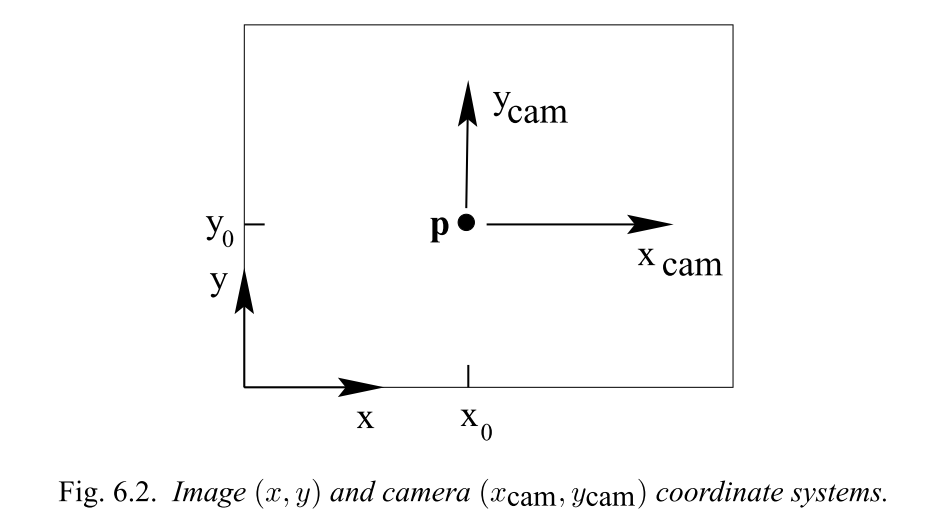
\includegraphics[width=\linewidth,natwidth=640,natheight=640]
  {fig/unofficial/pinhole_offset.png}
	\caption{Principle Point Offset}
	\label{fig:pinhole_offset}
\end{figure}

Thus, we get offsets, which can further be added into our function:

\begin{equation}
  \begin{pmatrix}
    U\\
    V\\
    1
  \end{pmatrix}
  =
  \begin{pmatrix}
    (f_xX + Z c_x)/Z\\
    (f_yY + Z c_y)/Z\\
    1
  \end{pmatrix}
  =
  \begin{pmatrix}
    f_xX + Z c_x\\
    f_yY + Z c_y\\
    Z
  \end{pmatrix}
  =
  \begin{bmatrix}
    f_x & 0 & c_x & 0\\
    0 & f_y & c_y & 0\\
    0 & 0 & 1 & 0\\
  \end{bmatrix}
  \begin{pmatrix}
    X\\
    Y\\
    Z\\
    1
  \end{pmatrix}
\end{equation} \label{eq:proj_1}

where $c_x$ and $c_y$ are coordinates of the principal point \textbf{p}.

\# Talk about square pixels and skew paramater.

\begin{equation}
  \begin{pmatrix}
    U\\
    V\\
    1
  \end{pmatrix}
  =
  \begin{bmatrix}
    \alpha_x & s & c_x & 0\\
    0 & \alpha_y & c_y & 0\\
    0 & 0 & 1 & 0\\
  \end{bmatrix}
  \begin{pmatrix}
    X\\
    Y\\
    Z\\
    1
  \end{pmatrix}
\end{equation} \label{eq:proj_2}


Then, we extract $\mathbf{K}$ matrix:

\begin{equation}
  \mathbf{K} = 
  \begin{bmatrix}
    \alpha_x & s & c_x\\
    0 & \alpha_y & c_y\\
    0 & 0 & 1\\
  \end{bmatrix}
\end{equation} \label{eq:k_matrix}

The $K$ is called \textit{intrinsic parameters matrix}. Now, we can further 
simplify it by applying the following substitution:

\begin{equation}
  U_{img} = K[I|0]X_{cam}
\end{equation} \label{eq:simplfied_proj_func}

\begin{equation}
  R_x(\theta) = 
  \begin{bmatrix}
    1 & 0 & 0\\
    0 & cos\theta & -sin\theta\\
    0 & sin\theta & cos\theta
  \end{bmatrix}
\end{equation}

\begin{equation}
  R_y(\theta) = 
  \begin{bmatrix}
    cos\theta & 0 & -sin\theta\\
    0 & 1 & 0\\
    sin\theta & 0 & cos\theta
  \end{bmatrix}
\end{equation}

\begin{equation}
  R_z(\theta) = 
  \begin{bmatrix}
    cos\theta & -sin\theta & 0\\
    sin\theta & cos\theta & 0\\
    0 & 0 & 1
  \end{bmatrix}
\end{equation}

\begin{equation}
  \mathbf{R} = \mathbf{R_z(\gamma)}\mathbf{R_y(\beta)}\mathbf{R_x(\alpha)}
\end{equation}

\begin{equation}
  \mathbf{t} = 
  \begin{bmatrix}
    t_x \\ t_y \\ t_z
  \end{bmatrix}
\end{equation}

\begin{equation}
  \begin{pmatrix}
    U\\
    V\\
    1
  \end{pmatrix}
  =
  \begin{bmatrix}
    \alpha_x & s & c_x & 0\\
    0 & \alpha_y & c_y & 0\\
    0 & 0 & 1 & 0\\
  \end{bmatrix}
  \begin{bmatrix}
    r_{11} & r_{12} & r_{13} & t_x\\
    r_{21} & r_{22} & r_{23} & t_y\\
    r_{31} & r_{32} & r_{33} & t_z\\
  \end{bmatrix}
  \begin{pmatrix}
    X\\
    Y\\
    Z\\
    1
  \end{pmatrix}
\end{equation} \label{eq:proj_1}



where $F(X_{cam})$ is the \textit{projection function}, which takes 
the 3D points in the Camera Coordinate System and maps them into the Image 
Coordinate Systems.



\subsection{Camera Calibration} \label{sb_sc_calibration}

\section{Image Features} \label{sc_img_features}

\section{Feature Matching} \label{sc_feature_matching}

\section{Motion Estimation} \label{sc_motion_estim}

% ***************************CP3-MOTIVATION***************************
\chapter{Motivation} \label{cp_motivation}

% ***************************CP4-CoVO***************************
\chapter{An Error-Aware RGB-D Visual Odometry} \label{cp_covo}

REMEMBER TO DRAW X,Y COORD. WRT CAM. COORD WITH RIGHT HAND FOR KINECT!

\section{Modeling Spatial Uncertainty} \label{sc_spatial_uncertainty}

\subsection{Kinect Calibration} \label{sb_sc_kinect_calibration}

\section{Weighted Least-Squares Optimization} \label{sc_weighted_lsq}

\section{Covariance Estimation} \label{sc_covariance_estim}

% ***************************CP5-EVALUATION***************************
\chapter{Evaluation} \label{cp_evaluation}

% ***************************CP6-CONCLUSION***************************
\chapter{Conclusion} \label{cp_conc}

% ***************************CP7-EVALUATION***************************
\chapter{Reference} \label{cp_ref}


% ***************************CP7-EVALUATION***************************
\chapter{Appendices} \label{cp_appendices}

\end{document}


